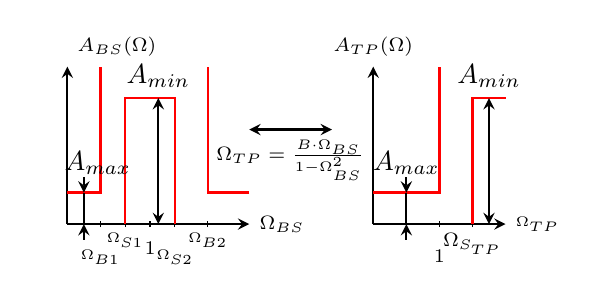
\begin{tikzpicture}[xscale=0.21, yscale=0.2]
% BS
\begin{scope}[local bounding box=BS]
	% Achsen zeichnen
	\draw[-{stealth},thick] (0,0) -- (11,0) node[right] {\scriptsize{$\Omega_{BS}$}};
	\draw[-{stealth},thick] (0,0) -- (0,10) node[above right] {\scriptsize{$A_{BS}(\Omega)$}};
	% Achsen beschriften
	\draw (2,-.2) -- (2,.2) node[below=7pt] {\tiny{$\Omega_{B1}$}};
	\draw (3.5,-.2) -- (3.5,.2) node[below=1pt] {\tiny{$\Omega_{S1}$}};
	\draw (5,-.2) -- (5,.2) node[below=4pt] {\scriptsize{$1$}};
	\draw (6.5,-.2) -- (6.5,.2) node[below=7pt] {\tiny{$\Omega_{S2}$}};
	\draw (8.5,-.2) -- (8.5,.2) node[below=1pt] {\tiny{$\Omega_{B2}$}};
	% BP-Teil zeichnen:
	\draw[color=red, thick] (0,2) -- (2,2) -- (2,10);
	\draw[color=red, thick] (3.5,0) -- (3.5,8) -- (6.5,8) -- (6.5,0);
	\draw[color=red, thick] (11,2) -- (8.5,2) -- (8.5,10); 
	\draw[{stealth}-{stealth}, thick] (5.5,0) -- (5.5,8) node[above] {$A_{min}$};
	\draw[-{stealth}, thick] (1,-1) -- (1,0);
	\draw[{stealth}-, thick] (1,2) -- node[above] {$\quad A_{max}$}(1,3);
	\draw[thick] (1,0) -- (1,2);
\end{scope}

% Verbindungspfeil
\begin{scope}[local bounding box=Pfeil, right of = BP]
\draw[{stealth}-{stealth}, thick] (10,6) -- node[below] {\scriptsize{$\Omega_{TP} = \frac{B\cdot\Omega_{BS}}{1 - \Omega_{BS}^2}$}}(15,6);
\end{scope}

% TP
\begin{scope}[local bounding box=TP,right of = Pfeil]
% Achsen zeichnen
\draw[-{stealth},thick] (17.5,0) -- (25.5,0) node[right] {\tiny{$\Omega_{TP}$}};
\draw[-{stealth},thick] (17.5,0) -- (17.5,10) node[above] {\scriptsize{$A_{TP}(\Omega)$}};
% Achsen beschriften
\draw (21.5,-.2) -- (21.5,.2) node[below=7pt] {\scriptsize{$1$}};
\draw (23.5,-.2) -- (23.5,.2) node[below=1pt] {\scriptsize{$\Omega_{S_{TP}}$}};
% TP-Teil zeichnen:
\draw[color=red, thick] (23.5,0) -- (23.5,8) -- (25.5,8);
\draw[color=red, thick] (17.5,2) -- (21.5,2) -- (21.5,10); 
\draw[{stealth}-, thick] (19.5,2) -- node[above] {$A_{max}$}(19.5,3);
\draw[-{stealth}, thick] (19.5,-1) -- (19.5,0);
\draw[{stealth}-{stealth}, thick] (24.5,0) -- (24.5,8) node[above] {$A_{min}$};
\draw[thick] (19.5,0) -- (19.5,2);
\end{scope}
\end{tikzpicture}